In this section, we focus on the algorithm details for the COCIS problems. COCIS is a joint optimization of coflow and OCS network to minimize the CCT. As we can see in \ref{sec:objective}, not only COCIS but also two subproblems of COCIS are NP-hard. In view of the complexity and difficulty of the COCIS problem, we separate our framework into two steps, which will be introduced in \ref{sec:framework}.

The rest of the algorithm section is organized as follows. Section \ref{sec:framework} shows the overall framework of our algorithm. In section \ref{sec:alg_coflow}, we introduce the first step our framework, which aims at coflow routing and scheduling. Section \ref{sec:alg_circuit} introduces the second step of our framework. Finally, section \ref{discussion} discusses some other things about our algorithms.
\subsection{Framework}\label{sec:framework}
In this part, we give the overall description of our framework. We separate our framework into two steps. First, we determine the route from the $k$ feasible lightpath set and the order distribution of each flow in the same lightpath. Second, given the route and duration of each lightpath, we schedule the circuits in the OCS network. Our framework is shown in Alg. \ref{alg:framework}.
{\small
\begin{algorithm}
\caption{ Framework     }\label{alg:framework}
\begin{algorithmic}[1]
%\STATE {\textbf{Input: }
\STATE {\textbf{Step 1:Coflow Routing and Order Distribution} /*  determine a lightpath for each flow in coflow $C$ and the order for flows in the same lightpath */ }

\STATE {\textbf{Step 2: Circuits Scheduling for Each Lightpath} /* assign each lightpath an active time whose length is the duration in step 1 */ }

\end{algorithmic}
\end{algorithm}
}


The first step is coflow routing and order distribution. It aims at scheduling the coflow. Each flow has $k$-feasible lightpaths and coflow routing will determine which lightpath the flow will pass through. That is, our coflow scheduling includes routing and order distribution. If multiple flows pass through the same lightpath, the forwarding order is another problem. It's what the order distribution does. After appointing all the flows in $C$, we will compute the duration of each lightpath, which is the input of step 2. The second step in the framework get the duration of each lightpath. It will schedule the circuits of the whole network to minimize the CCT and output the scheduling scheme. Each lightpath will have an active period whose interval length is its duration. Because step 2 appoints each lightpath the exact duration. So the order in the same lightpath can be changed. That is, we only need to know the duration of each ligthpath. However, in the practical implementation of step 1, we do have an order for each flow to get a better approximation performance.
%\subsection{Approximation Bound Analysis for IRSC}


%\subsection{Non-Interruptible Routing and Scheduling for Coflows (NIRSC)}
\subsection{Greedy Routing and Order Distribution (GROD)\& Analysis }\label{sec:alg_coflow}
We introduce step 1 of our framework. Given the Coflow $C$ and the feasible lightpath set for a source-destination ToR pair, we assign each ligthpath a number of flows with an greedy algorithm. There might be an exponential number of feasible lightpaths between a source ToR switch and a destination ToR switch. Following \cite{hong2013achieving} \cite{al2010hedera}, we assume that the central scheduler has pre-computed $k$ feasible lightpaths between each pair of ToR switches corresponding to the $k$ output port of a ToR switch. Note that $P=\bigcup_{i,j}P_{i,j}$ is the feasible lightpath set of the network. For a coflow, the algorithm will be executed iteratively until all the source-destination ToR pairs are traversed. It's worth noting that the routes of feasible lightpaths are ensured and the circuits scheduling that makes lightpaths active is the responsibility of step 2. There is a flow set for each ToR pair, for example, $\Gamma_{i,j}$. Without loss of generality, we use ToR pair $(i,j)$ and flow set $\Gamma_{i,j}$ as an example. For flow set $\Gamma_{i,j}=\{f_{i,j}^1,f_{i,j}^2,...f_{i,j}^m\}$ and feasible lightpath set $P_{i,j}=\{p_{i,j}^1,p_{i,j}^2,...,p_{i,j}^k\}$, the first step sorts all flows in $\Gamma_{i,j}$ non-increasingly according to their amount of data. In the second step, for each flow $f\in \Gamma_{i,j}$, appoint $f$ to the lightpath with the least duration. duration of a lightpath means the total processing time to forward the flows. Finally, the lightpath that is appointed a new flow will update the duration. The GROD algorithm outputs the required duration for each lightpath. The duration matrix is denoted by $T=\{t_{i,j,l}\}$.

{\small
\begin{algorithm}
\caption{GROD: Greedy Routing and Duration Assignment}\label{alg:GROD}
\begin{algorithmic}[2]
\STATE {\textbf{Input: $C$, $P_{i,j},\forall i,j$}}
\STATE {\textbf{Output: Duration Matrix $T$}}

%\STATE {\textbf{Step 1:Route and Duration Assignment (RDA) for Each Flow} /* for each flow in coflow $C$, determine a lightpath*/ }
\FOR {each $\Gamma_{i,j}\in C$}
    %\STATE {\textbf{Step 1:Route and Duration Assignment (RDA) for Each Flow}/* for each flow in coflow $C$, determine a lightpath*/ }
    \STATE {Initiate duration array $T_{i,j}\ =0$ for each element.}
    \STATE {Sort all flows in $\Gamma_{i,j}$ non-increasingly according to their amount of data}
    \FOR {each $f\in \Gamma_{i,j}$}
         \STATE {Assign the flow to the lightpath with the least duration in $P_{i,j}$}
         \STATE {Update the duration of the lightpath }
    \ENDFOR
\ENDFOR
%\STATE {\textbf{Step 1: For a fixed OCS network scheduling scheme, we construct an interruptible/non-interruptible routing and scheduling algorithm }}
%\STATE {\textbf{Step 2: Circuits Scheduling (CIS) for Each Lightpath} /*assign each lightpath an active time whose length is the duration in step 1*/ }

\end{algorithmic}
\end{algorithm}
}


\textbf{Approximation Bound Analysis for GROD.} We analyze the approximation performance of the proposed GROD algorithm. Because GROD is executed iteratively, the approximation bound will be the same for each source-destination ToR switch pair.  Without loss of generality, we use a source-destination ToR swtich pair $(i,j)$ as an example. Note that $GROD(I)$ is the maximum duration for $k$ lightpaths in $P_{i,j}$ with GROD and $OPT(I)$ is the optimal result when the input flow set is $I$. The approximation ratio is $R_{GROD}$.

\begin{theorem}\label{bound:GROD}
The approximation ratio $R_{GROD}\leq\frac{4}{3}-\frac{1}{3k}$.
\end{theorem}
\begin{IEEEproof}
If $k=1$, because $GROD(I)=OPT(I)$ and $\frac{4}{3}-\frac{1}{k}=1=\frac{GROD(I)}{OPT(I)}$.

For $k>1$, we assume that $I=\{f_1,f_2,...,f_m\}$ is the flow set with the least flow number that contradicts to the approximation ratio. The amount of data for the flows is $\{d_1,d_2,....d_m\}$, and the duration of flows are $\{t_1,...,t_m\}$. Thus the scheduling order is $\{f_1,f_2,...,f_m\}$ and the maximum duration of each lightpath is $GROD(I)$. We set the last finished flow is $f_{m_1}$ and $m_1=n$. Because if $m_1<n$, there exists another flow set $I'=\{f_1,f_2,...,f_{m_1}\}$ whose maximum duration is also $GROD(I)$. That is $GROD(I')=GROD(I)$.  However, it's optimal result $OPT(I')\leq OPT(I)$. So we have:
\begin{equation}
\frac{GROD(I')}{OPT(I')}\geq\frac{GROD(I)}{OPT(I)}> \frac{4}{3}-\frac{1}{3k}
\end{equation}

The above equation contradicts to our assumption that $I$ is the flow set with the least flow number that contradicts to the approximation ratio, so $m_1=m$. Now, we prove that if $I$ exists, $m\leq 2k$.

Because $f_m$ is the last finished flow, $f_m$ starts at $GROD(I)-t_m$. At that time, this lightpath had the least duration. So we have:
\begin{equation}
\begin{aligned}
GROD(I)-t_m  &\leq\frac{1}{k}\sum\limits_{q=1}^{m-1}t_q\\
GROD(I) &\leq\frac{1}{k}\sum\limits_{q=1}^{m}t_q+\frac{k-1}{k}t_m\\
\end{aligned}
\end{equation}

Combined with $OPT(I)\geq \sum\limits_{q=1}^{m}t_q$, we have:

\begin{equation}
\begin{aligned}
&\frac{4}{3}-\frac{1}{3k}\leq \frac{GROD(I)}{OPT(I)}\leq\frac{OPT(I)+\frac{k-1}{k}t_m}{OPT(I)}\\%=1+\frac{k-1}{k}\frac{t_m}{OPT(I)}\\
&\Rightarrow 4k-1<3k+3(k-1)\frac{t_m}{OPT(I)}\\
& \Rightarrow\ OPT(I)<3t_m
\end{aligned}
\end{equation}

Because $t_m$ is the least number among $\{t_1,...,t_m\}$, $m<2k$. Furthermore, we proof GROD is the optimal solution when $m<2k$. We set $m=2k$, since if $m\ne2k$, we set $t_q=0,\forall q=m+1,..,2k$. We set assume lightpath has two flows: $f_x$ and $f_y$. If $x,y\leq k$, there exists a lightpath whose two flows are $f_s,f_t,s,t>k$. Because $t_x,t_y\geq t_s,t_t$, we swap $t_y$ and $t_t$. Then $t_x+t_t\leq t_x+t_y$ and $t_s+t_y\leq t_x+t_y$. The scheduling scheme $O'$ after the swap is no big than the optimal solution, so $O'$ is an optimal solution too. For scheduling scheme $O'$, $f_1,...f_k$ are appointed to the $k$ different feasible lightpaths, so do $f_{k+1},...f_{2k}$. The scheduling scheme is the same as the GROD algorithm. So we have:
\begin{equation}
\frac{GROD(I)}{OPT(I)}=1\leq\frac{4}{3}-\frac{1}{3k}(k\geq2)
\end{equation}

In conclusion, on one hand, when $m=1$, GROD is the optimal solution, so the approximation ratio is $1$. On the other hand, when $m\geq2$, if there exists a counterexample $I$, $m$ must be no more than $2k$. Furthermore, we show GROD is the optimal solution if $m\leq2k$. We have proven that the counterexample $I$ doesn't exist, so lemma \ref{bound:GROD} is proved.
\end{IEEEproof}
\subsection{Circuits Scheduling \& Analysis}\label{sec:alg_circuit}
After the first step of the framework, we get the output: Duration matrix $T=\{t_{i,j,l}\}$. $t_{i,j,l}$ represents the duration of $l^{th}$ lightpath in $P_{i,j}$. In this section, we schedule the circuits in the OCS network to minimize the coflow completion time. Because the circuits scheduling will change the status of ports and lightpaths dynamically, we keep a table holding information about each lightpath and port of when they are free or busy, denoted by NST (Network Status Table). Once a port is released, we will search the lightpath set to find whether there exists a lightpath $p_{i,j,l}$ along which the ports are all free or not. If so, we will take up the ports and forward the flows until all the flows appointed to the lightpath are forwarded. What's more, lightpath $p_{i,j,l}$ will be excluded from the lightpath set and the NST will change the status of the lightpath $p_{i,j,l}$ and corresponding ports. Their status will be busy for the duration $t_{i,j,l}$. If not, we will wait until the next port is released. Our algorithm terminates when all the lightpath is excluded from lightpath set. Obviously, our loop can end because if there is lightpath remain in the lightpath set, it can at least wait until all the ports are free. Our circuits scheduling algorithm is given in Alg. \ref{alg:CIS}.
\begin{table}[!tp]
\begin{tabular}{c|c}
\hline
\hline
B& bandwidth of the link\\
\hline
$P\{p_{i,j,l}\}$&feasible lightpath set for all the ToR pairs\\
\hline
NST& Network Status Table\\
\hline
$Start(.)$& the start time of a lightpath\\
\hline
$End(.)$& the end time of a lightpath \\
\hline
$T=\{t_{i,j,l}\}$& duration matrix for the lightpath set $P$\\
\hline
$\delta$ &the reconfiguration time \\
\hline
$T_L$ &lower bound for the CCT\\
\hline
$T_O$ &CCT of optimal solution\\
\hline
$\Delta t_i$ &idle interval between $p_{i-1}$ and $p_i$\\
\hline
$h$ &the maximum hop count of lightpaths\\
\hline
\end{tabular}
\caption{Some Important Notations for Section \ref{sec:alg_circuit}}\label{tbl:notation}
\end{table}

\textbf{Approximation Bound Analysis for CIS.} Next, we analyze the circuits scheduling performance. In order not to conflict with the whole paper, \textbf{new notions in this section only suitable for this section}.

Before the analysis of approximation bound, we discuss the lower bound for our problem. For a port $j$, there are lightpath $p_1,p_2,...,p_N$ that pass through the port. Note that the transmission time is $t_1,...,t_1$. So the minimum time to finish the task is:
 \begin{equation}\label{eq:T_L}
 T_L^j=\sum\limits_{i=1}^{N}t_i
 \end{equation}

\begin{algorithm}
\caption{CIS: Circuits Scheduling Algorithm}\label{alg:CIS}
\begin{algorithmic}[3]
	\STATE $t$ = Begin time
	\WHILE{$P\ne \varnothing$}
	\FOR {$p_{i,j,l}$ in $P$}
	\STATE $temp=\delta+t_{i,j,l}$
	\STATE Search NST for all ports along the lightpath $P_{i,j,l}$
	\IF {all ports along $P_{i,j,l}$ is free at time $t$}
	\STATE Arrange lightpath $p_{i,j,l}$ to start at $t$ :
	\STATE $Start(p_{i,j,l})=t$
	\STATE $End(p_{i,j,l})=t+temp$
	\STATE Set lightpath $p_{i,j,l}$ is busy during $t$ to $t+temp$ in NST
	\FOR {each ports $p$ along the lightpath $p_{i,j,l}$}
	\STATE Set $p$ is busy during $t$ to $t+temp$ in NST
	\ENDFOR
	\STATE $P=P-p_{i,j,l}$
	\ENDIF
	\ENDFOR
	\STATE $t=$the next nearest release time in NST
	\ENDWHILE
\end{algorithmic}
\end{algorithm}



Note that the lower bound is $T_L$. we have:
\begin{equation}
T_L=\max\{T_L^1,T_L^2,...,\}
\end{equation}

\begin{theorem}\label{bound:CIS}
Algorithm CIS completes the transmission within $h$ times of the optimal solution, where $h$ is the maximum hop count of all the lightpaths.
\end{theorem}
\begin{IEEEproof}
Because a link connects to two ports, one input port and one output port, we use input port $j$ as an example. sort the lightpaths that pass through input port $j$ by the time they are scheduled to start transmission, denoted by $p_1,...,p_N$. $t_i$ denotes the time to transmit (including the reconfigure time delay $\delta$), and $\Delta t_i$ represents the idle interval between $p_{i-1}$ and $p_i$.

During $\Delta t_i$, port $j$ is idle. According to our algorithm, it means links of lightpath $f_i,f_{i+1},...,f_N$ are all busy during $\Delta t_i$ and at least one port of each lightpath is transmitting data for other lightpaths. Consider the last lightpath $p_N$, it has waited for $\sum\limits_{i=1}^{N}\Delta t_i$ totally. During the waiting time, the worst case is that all input ports, except port $j$, have finish their task. Combined with the lower bound, we know that a port finishes its task within $T_L$. Note that lightpath $p_N$ has $h_N$ input ports. We have:
\begin{equation}
\sum\limits_{i=1}^{N}\Delta t_i\leq (h_N-1)T_L\leq(h-1)T_L
\end{equation}


\begin{figure}
	\centering
    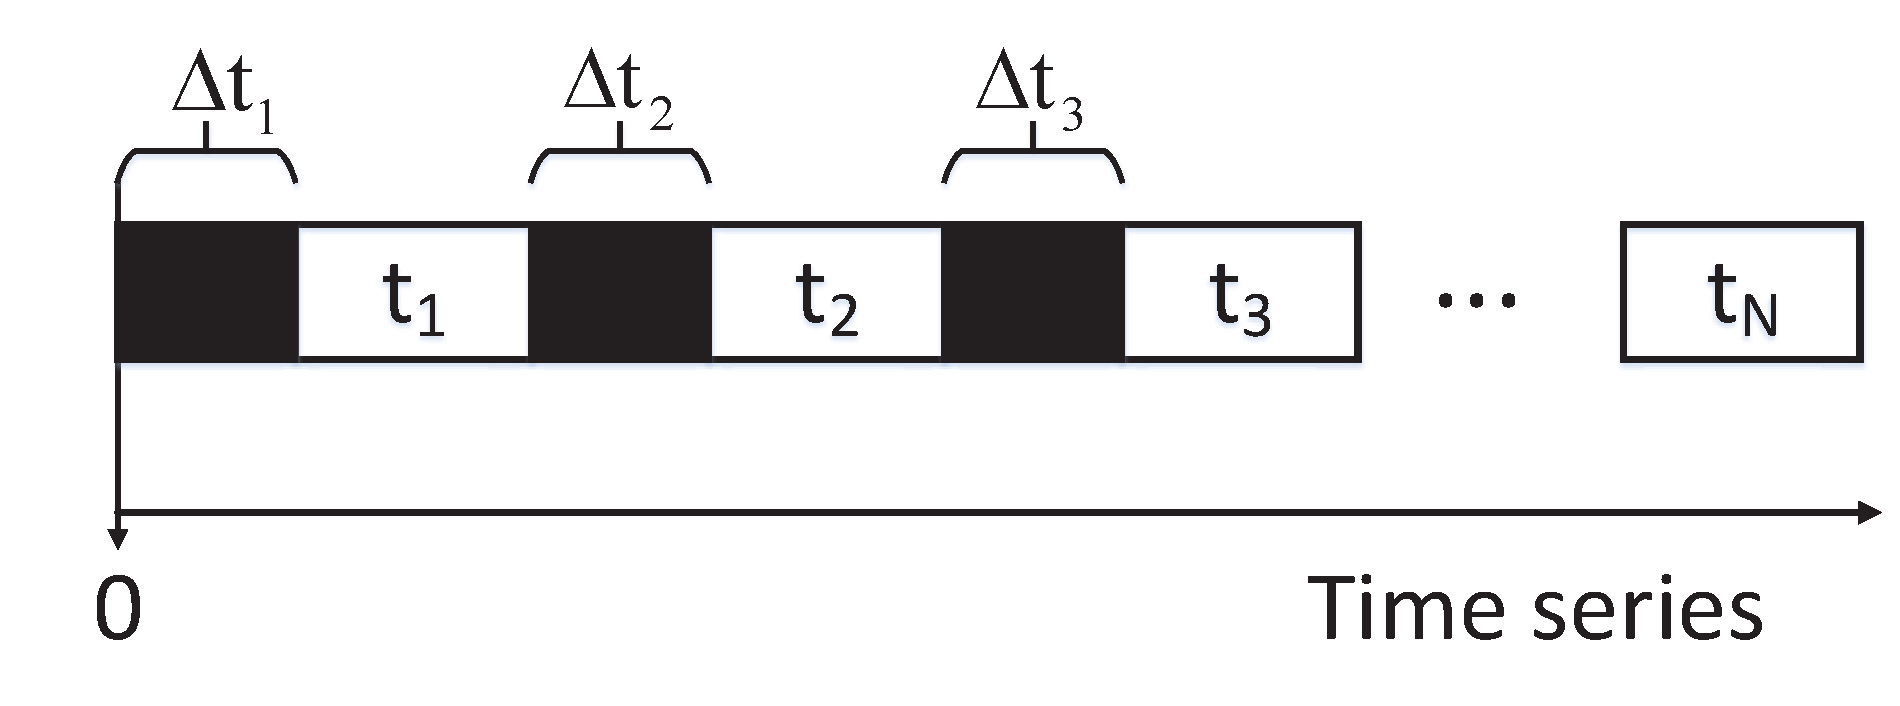
\includegraphics[width=0.45\textwidth]{timeline.eps}
	\caption{Timeline of a port}\label{fig:timeline}
\end{figure}

The transmission time of port $j$ is $\sum\limits{i=1}^N t_i$. According to Eq. \ref{eq:T_L}, we know:
\begin{equation}
\sum\limits_{i=1}^N t_i\leq T_L
 \end{equation}

So the completion time for port $j$ is:
\begin{equation}
\sum\limits_{i=1}^N t_i+\sum\limits_{i=1}^{N}\Delta t_i\leq (h-1)T_L+T_L=h T_L
\end{equation}

The completion time of the optimal solution is denoted by $T_O$. Because $T_L$ is lower bound to transmit the task, we have:
\begin{equation}
T_L<T_O
\end{equation}

The port $j$ is arbitrary, so algorithm CIS completes the transmission within $h$ times of the optimal solution. Lemma \ref{bound:CIS} is proved.

\end{IEEEproof}

\subsection{Time Conplexity}
In this section, we analyze the time complexity of GROD and CIS.

\begin{theorem}\label{time:GROD}
GROD's time complexity is $O(|\Gamma|\log m)$, where $m$ is the number of flows for each ToR switch pair.
\end{theorem}
\begin{IEEEproof}
GROD is executed for each ToR switch pair. For each pair $(i,j)$, there is a flow set $f_{i,j}$ and $|f_{i,j}|=m$. We sort the flow set with time complexity $O(m\log m)$, then appoint the flow with time complexity $O(m)$. So the total time complexity is $O(|\Gamma|(\log m+1))=O(|\Gamma|\log m )$.
\end{IEEEproof}
\begin{theorem}\label{time:CIS}
CIS's time complexity is $O(h|P|^2)$. Where $h$ is the maximum hop count of lightpaths.
\end{theorem}
\begin{IEEEproof}
The first loop is for all lightpaths in $P$. In the first loop, we first check the ports along the lightpath with time complexity $O(|P|h)$. After that we will go into the secong loop for all the lightpaths in $P$ with time complexity $O(|P|^2)$. In the second loop, we will check the ports along the lightpath with time complexity $O(h|P|^2)$. So the time complexity is $O(h|P|^2)$.
\end{IEEEproof}
\subsection{Discussion}\label{discussion}
The previous GROD and CIS algorithms are for intra-coflow scheduling. In this section, we will discuss inter-coflow scheduling. When multiple coflows compete for network resource, an important goal is to accommodate the network resource management policies for these coflows.

However, under different usage scenarios, we may need to use different management policies. For example, the policy may require that coflow requested by privileged users are preferred over that of regular users. Another example is that the policy may require the later-staged coflows yield to earlier-staged coflows to avoid the potential creation of stragglers that unnecessary prolong job runtime \cite{chowdhury2015efficient}. So the management is flexible and dependent on different constraints and objectives.

On the other hand, our GROD algorithm has already computed the required duration of each lightpath, and the CIS assign the lightpath the exact required duration. if we add a new task from another coflow, it may change the NST and furthermore increase the CCT of the original coflow. An stable way is to run each intra-coflow in order like \cite{huang2016sunflow}, which is one of the only a few researches that discussed the inter-coflow scheduling.
%\subsection{Approximation Bound Analysis for NIRSC}
